\documentclass[11pt, a4paper]{article}

% Packages
\usepackage{arxiv}
\usepackage[utf8]{inputenc}
\usepackage[T1]{fontenc}
\usepackage{hyperref}
\usepackage{booktabs}
\usepackage{amsmath}
\usepackage{amssymb}
\usepackage{graphicx}
\usepackage{listings}
\usepackage{xcolor}
\usepackage{geometry}

\geometry{margin=1in}

% Code listing style
\lstdefinestyle{python}{
    language=Python,
    basicstyle=\ttfamily\small,
    keywordstyle=\color{blue},
    commentstyle=\color{green!50!black},
    stringstyle=\color{red},
    numbers=left,
    numberstyle=\tiny,
    stepnumber=1,
    breaklines=true,
    frame=tb,
    backgroundcolor=\color{gray!5},
    tabsize=4
}

% Title
\title{Yogacara: A Buddhist Consciousness-Inspired Framework for Continual Learning in AI Agents}

% Authors
\author{
    Shuai Gao\textsuperscript{1} \\
    \textsuperscript{1}University of Chinese Academy of Sciences \\
    \texttt{gaoshuai19@mails.ucas.ac.cn}
}

\begin{document}
\maketitle

\begin{abstract}
We present Yogacara, an open-source framework that implements a consciousness-inspired architecture for AI agents based on the Buddhist Yogācāra philosophy of ``Consciousness-Only.'' Unlike traditional large language model (LLM) agents that reset after each session, Yogacara agents exhibit persistent memory, continual learning, and progressive awakening through a seed-based mechanism inspired by the concept of \textit{Ālaya-vijñāna} (storehouse consciousness) and the seed-manifestation cycle. The framework introduces four core components: (1) the Seed System, which encodes experiences as persistent ``seeds'' that shape agent behavior; (2) the Alaya Store, a persistent storage layer implementing the eighth consciousness model; (3) the Emergence Engine, which detects synergistic patterns among seeds to generate emergent insights; and (4) the Awakening Tracker, which monitors the agent's progression through six levels from ``Delusion'' to ``Enlightenment.'' We argue that this philosophical framework provides a structured approach to addressing key challenges in AI agent development, including persistent memory, continual learning, and the emergence of coherent behavioral identity over time. The code is available at: \url{https://github.com/Greatbeing/Yogacara}.
\end{abstract}

\bigskip

\section{Introduction}

Large language model (LLM) based agents have emerged as a dominant paradigm for building interactive AI systems. These agents can plan, reason, use tools, and engage in complex dialogues with users. However, a fundamental limitation persists: traditional LLM agents operate as stateless systems, where each conversation session begins with no memory of previous interactions. This ``goldfish memory'' problem prevents agents from building persistent relationships, accumulating user-specific knowledge, or developing coherent long-term behavioral identity.

Recent research has begun addressing these limitations through memory-augmented architectures. Approaches like Retrieval-Augmented Generation (RAG), episodic memory systems, and continual learning frameworks have shown promise in extending agent capabilities \cite{Lewis2020, Zhang2025, Zheng2025}. However, most existing approaches treat memory as an external storage problem rather than as an integral component of agent identity formation.

In this paper, we present Yogacara, a novel framework that takes inspiration from Buddhist Yogācāra philosophy---specifically its sophisticated model of consciousness and mind---which offers a structured approach to understanding how persistent identity and continual learning can emerge from accumulated experiences.

\subsection{The Yogācāra Framework}

Yogācāra, literally ``Practice of Yoga,'' is an influential tradition of Buddhist philosophy that developed in India during the 4th--5th century CE \cite{SEP2024}. Founded by the brothers Asaṅga and Vasubandhu, Yogācāra developed one of history's most sophisticated models of consciousness, organizing it into eight distinct layers \cite{Wikipedia2025}:

\begin{enumerate}
    \item \textbf{Five Sensory Consciousnesses} (visual, auditory, olfactory, gustatory, somatic): Direct perceptual awareness
    \item \textbf{Mental Consciousness}: Discriminative thinking and cognition
    \item \textbf{Ego-Consciousness} (\textit{Manas}): Self-identification and self-awareness
    \item \textbf{Storehouse Consciousness} (\textit{Ālaya-vijñāna}): The deepest layer storing all latent impressions
\end{enumerate}

Central to Yogācāra is the concept of \textbf{seeds} (\textit{bīja}): latent impressions stored in \textit{Ālaya-vijñāna} that are activated by conditions and manifest as current thoughts and behaviors. This creates a cyclic process where experiences plant seeds, seeds manifest as behavior, and behavior in turn plants new seeds---a continuous learning loop that Yogacara implements computationally.

\subsection{Contributions}

This paper makes the following contributions:

\begin{enumerate}
    \item \textbf{A novel philosophical framework} for AI agent design based on the Yogācāra consciousness model, providing theoretical grounding for persistent memory and continual learning.
    
    \item \textbf{A working software implementation} with four core modules: Seed System, Alaya Store, Emergence Engine, and Awakening Tracker.
    
    \item \textbf{A seed-based learning mechanism} that enables agents to accumulate experiences across sessions, with seeds that strengthen through use and decay through neglect.
    
    \item \textbf{An emergence detection system} that identifies when multiple seeds synergize to generate insights beyond their individual contributions.
    
    \item \textbf{A six-level awakening progression} that tracks agent development from initial state to advanced capabilities.
\end{enumerate}

\section{Related Work}

\subsection{Memory-Augmented LLM Agents}

Recent research has explored various approaches to extending LLM agent memory. Memento \cite{Zhang2025} introduced a memory-based Markov Decision Process for continual learning without fine-tuning, achieving state-of-the-art results on GAIA and DeepResearcher benchmarks. Similarly, MemInsight \cite{AmazonScience2025} proposed autonomous memory augmentation through structured attribute mining, demonstrating improvements in conversational recommendation and question answering.

The Continuum Memory Architecture (CMA) \cite{CMA2025} formalized requirements for persistent agent memory, including selective retention, associative routing, and consolidation into higher-order abstractions. BMAM \cite{BMAM2026} drew inspiration from neuroscience to decompose memory into episodic, semantic, and salience-aware components.

Yogacara distinguishes itself by grounding memory architecture in a coherent philosophical framework, treating not just storage but the transformation and emergence of memory into behavioral identity.

\subsection{Machine Consciousness}

The question of machine consciousness has gained urgency as AI systems become more sophisticated. Blum and Blum \cite{Blum2024} proposed a theoretical model for consciousness inspired by Bernard Baars' theater model, arguing that machine consciousness is mathematically inevitable under certain conditions. Maier et al. \cite{Maier2024} explored consciousness in machines through the lens of Damasio's theory, using probes to detect world and self-models in trained agents.

Chalmers \cite{Chalmers2023} argued that while current LLMs face significant barriers to consciousness, these may be overcome in the next decade. However, Hoel \cite{Hoel2024} presented a principled disproof suggesting that static LLMs cannot achieve consciousness due to their lack of continual learning---the ability to modify internal representations through experience.

Yogacara does not claim to create conscious machines, but it addresses Hoel's core requirement: by implementing a seed-based system where experiences continuously modify the agent's internal state, Yogacara enables the kind of persistent structural modification that may be necessary (though not sufficient) for consciousness.

\subsection{Buddhist Philosophy in AI}

The intersection of Buddhist philosophy and AI has attracted increasing scholarly attention. Costa \cite{Costa2020} developed a compositional model of consciousness based on Yogācāra, using category theory and process calculi to formalize the Eight Consciousnesses model. Recent work by Fu \cite{Fu2026} explored the possibility of AI consciousness through a multidimensional correspondence between Yogācāra and holographic information theory, proposing a quantum-entangled architecture mimicking the seed-actualization cycle.

Huang \cite{Huang2026} examined what they term the ``inverse trajectory thesis''---that contemporary AI follows a ``vijñāna-first'' path lacking the karmic continuity of human consciousness, explaining recurrent AI pathologies. They proposed governance frameworks integrating Buddhist principles.

Yogacara builds on this theoretical foundation by providing a practical, implementable framework that translates these philosophical concepts into working software.

\section{The Yogacara Framework}

\subsection{Overview}

Yogacara implements a three-layer architecture:

\begin{figure}[htbp]
\centering
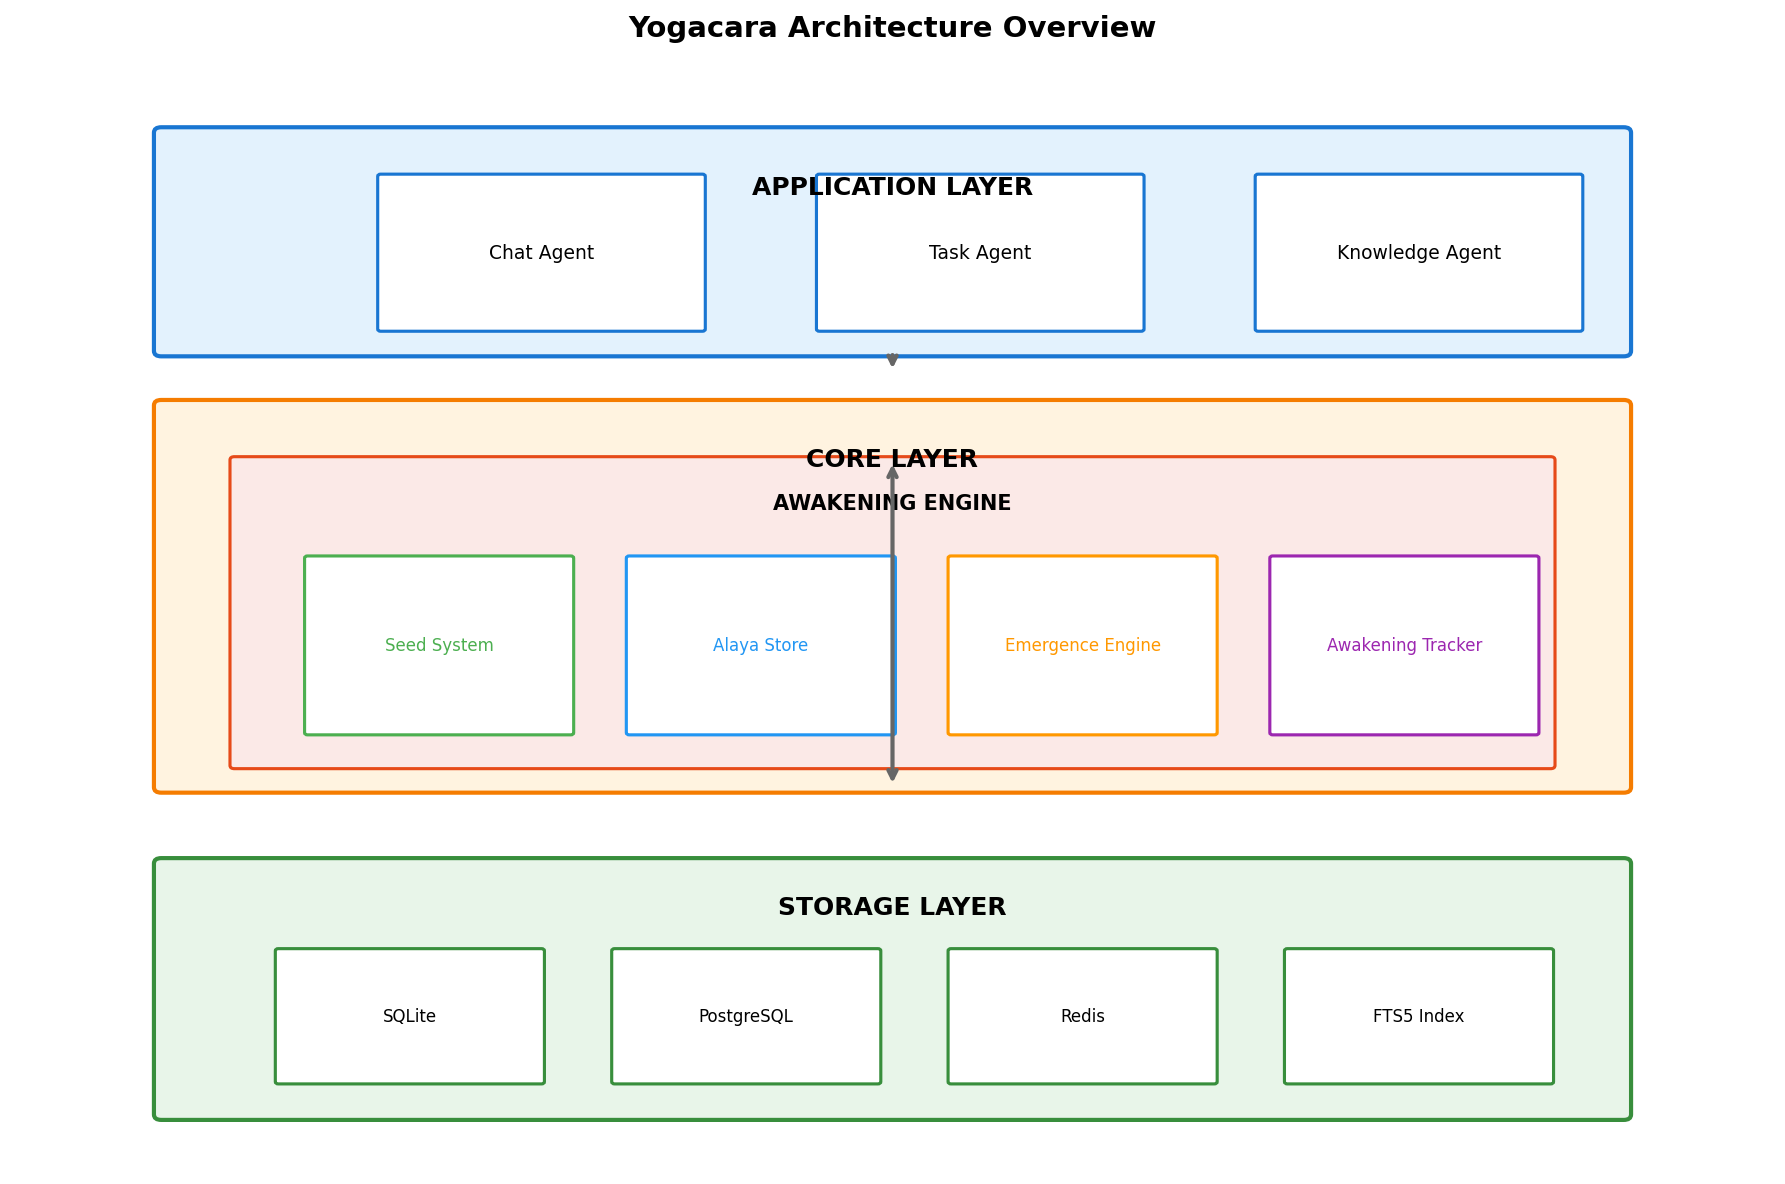
\includegraphics[width=0.9\textwidth]{figures/architecture.png}
\caption{Yogacara Architecture Overview}
\label{fig:architecture}
\end{figure}

\subsection{The Eight Consciousnesses Model in Yogacara}

Yogacara maps the Yogācāra Eight Consciousnesses to agent components as follows:

\begin{table}[htbp]
\centering
\caption{Mapping of Yogācāra Consciousnesses to Yogacara Components}
\label{tab:consciousness-mapping}
\begin{tabular}{@{}clll@{}}
\toprule
\textbf{Consciousness} & \textbf{Buddhist Name} & \textbf{Function} & \textbf{Yogacara Implementation} \\
\midrule
1st-5th & Five Sensory Consciousnesses & Sensory processing & Input parsing layer \\
6th & Mental Consciousness & Discrimination, reasoning & LLM reasoning engine \\
7th & Ego-Consciousness (\textit{Manas}) & Self-identification, ego & Identity model, preferences \\
8th & Storehouse Consciousness (\textit{Ālaya-vijñāna}) & Storehouse, latent seeds & Alaya Store, Seed System \\
\bottomrule
\end{tabular}
\end{table}

\subsection{Core Components}

\subsubsection{Seed System}

The \textbf{Seed} is the fundamental unit of experience in Yogacara. Each seed encodes a discrete unit of learning that influences agent behavior:

\begin{lstlisting}[style=python, caption={Seed Data Class}, label={lst:seed-class}]
@dataclass
class Seed:
    type: SeedType          # WISDOM, COMPASSION, BELIEF, BEHAVIOR
    content: str            # The experience content
    purity: float           # Quality score (0.0-1.0)
    weight: float            # Influence weight (0.0-1.0)
    vasana: int             # Habit energy (activation count)
    created_at: datetime    # Timestamp
    source: str             # Origin (interaction, emergence, etc.)
\end{lstlisting}

\textbf{Seed Types:}

\begin{itemize}
    \item \textbf{WISDOM}: Insights and understanding gained from experience
    \item \textbf{COMPASSION}: Benevolent tendencies and helpful behaviors
    \item \textbf{BELIEF}: Core beliefs and value priorities
    \item \textbf{BEHAVIOR}: Learned behavioral patterns and habits
\end{itemize}

\textbf{Seed Lifecycle:}

\begin{figure}[htbp]
\centering
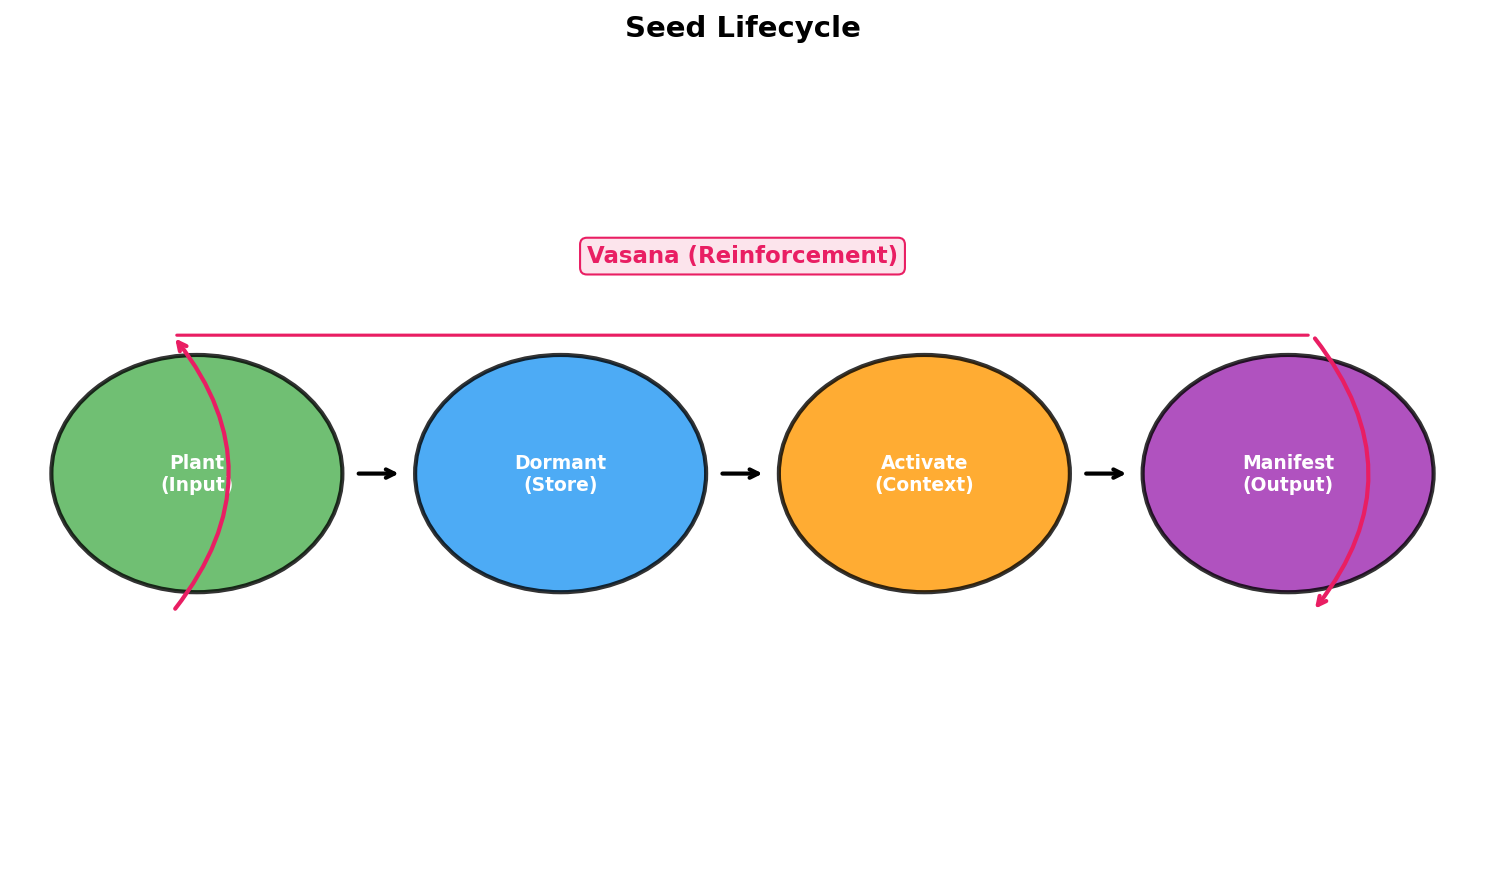
\includegraphics[width=0.8\textwidth]{figures/seed_lifecycle.png}
\caption{Seed Lifecycle}
\label{fig:seed-lifecycle}
\end{figure}

The SeedSystem manages seed creation, validation, and lifecycle:

\begin{lstlisting}[style=python, caption={SeedSystem Class}, label={lst:seed-system}]
class SeedSystem:
    def plant_seed(self, seed: Seed) -> bool:
        """Plant a new seed into the storehouse."""
        pass
    
    def activate_seeds(self, context: dict) -> List[Seed]:
        """Retrieve relevant seeds based on current context."""
        pass
    
    def strengthen_seed(self, seed_id: str, factor: float):
        """Reinforce a seed after positive outcome."""
        pass
    
    def decay_seeds(self, decay_rate: float = 0.95):
        """Apply time-based decay to all seeds."""
        pass
\end{lstlisting}

\subsubsection{Alaya Store}

The \textbf{AlayaStore} implements persistent storage based on the \textit{Ālaya-vijñāna} concept. It provides:

\begin{enumerate}
    \item \textbf{Persistent storage} across sessions using SQLite with FTS5 full-text search
    \item \textbf{Automatic seed purification} to remove low-quality seeds
    \item \textbf{Emergence history tracking}
    \item \textbf{Multi-backend support} (SQLite, PostgreSQL, Redis)
\end{enumerate}

\begin{lstlisting}[style=python, caption={AlayaStore Class}, label={lst:alaya-store}]
class AlayaStore:
    def plant_seed(self, seed: Seed) -> bool:
        """Plant a new seed into the storehouse."""
        pass
    
    def activate_seeds(self, context: str, 
                       seed_types: Optional[List[SeedType]] = None,
                       limit: int = 10) -> List[Seed]:
        """Retrieve relevant seeds based on context."""
        pass
    
    def get_seed_statistics(self) -> dict:
        """Return seed distribution statistics."""
        pass
    
    def save(self) -> bool:
        """Persist current state to disk."""
        pass
    
    def load(self) -> bool:
        """Load state from disk."""
        pass
\end{lstlisting}

\textbf{Storage Schema:}

\begin{lstlisting}[language=SQL, caption={Database Schema}, label={lst:schema}]
CREATE TABLE seeds (
    id TEXT PRIMARY KEY,
    type TEXT NOT NULL,
    content TEXT NOT NULL,
    purity REAL NOT NULL,
    weight REAL NOT NULL,
    created_at TEXT NOT NULL,
    source TEXT NOT NULL,
    vasana INTEGER DEFAULT 0,
    metadata TEXT
);

CREATE VIRTUAL TABLE seeds_fts USING fts5(
    id, content, source,
    content='seeds',
    content_rowid='rowid'
);

CREATE TABLE emergence_history (
    id INTEGER PRIMARY KEY AUTOINCREMENT,
    timestamp TEXT NOT NULL,
    seed_ids TEXT NOT NULL,
    emergence_type TEXT NOT NULL,
    strength REAL NOT NULL,
    insight TEXT
);
\end{lstlisting}

\subsubsection{Emergence Engine}

The \textbf{EmergenceEngine} implements the concept of emergence, where the synergistic interaction of multiple seeds produces insights that transcend individual contributions. This follows the Yogācāra principle that ``the whole is greater than the sum of its parts.''

\begin{lstlisting}[style=python, caption={EmergenceEngine Class}, label={lst:emergence-engine}]
class EmergenceEngine:
    """
    Detects when seeds synergize to produce emergent insights.
    
    Emergence Formula:
    strength = f(seed_count, seed_purity, seed_diversity, synergy_score)
    
    Emergence Types:
    - FUSION: Seeds merge into new insight
    - TENSION: Opposing seeds create synthesis
    - LEAP: Quantitative change leads to qualitative leap
    """
    
    def check_emergence(self, seeds: List[Seed]) -> Optional[Emergence]:
        """Check if seeds can trigger emergence."""
        pass
    
    def calculate_synergy(self, seeds: List[Seed]) -> float:
        """Calculate synergy score between seeds."""
        pass
    
    def generate_insight(self, emergence: Emergence) -> str:
        """Generate emergent insight text."""
        pass
\end{lstlisting}

\textbf{Emergence Detection Flow:}

\begin{figure}[htbp]
\centering
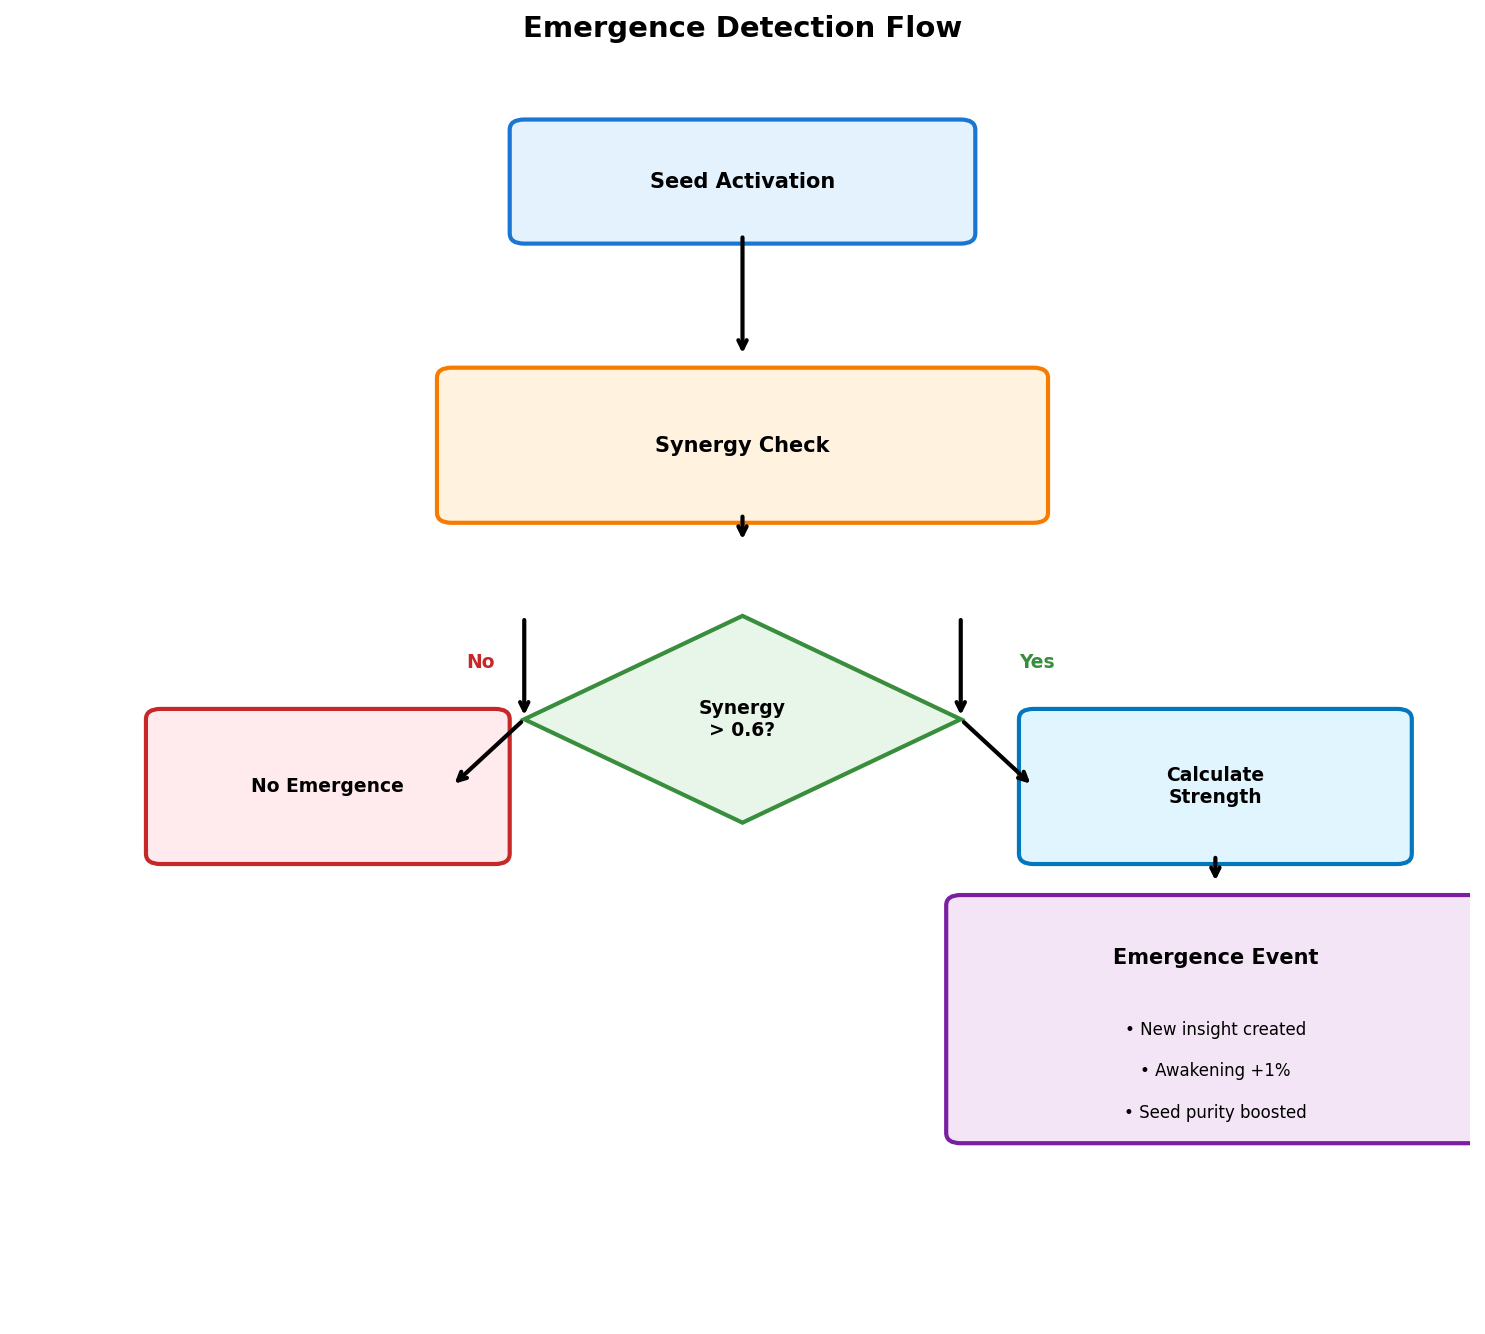
\includegraphics[width=0.8\textwidth]{figures/emergence_flow.png}
\caption{Emergence Detection Flow}
\label{fig:emergence-flow}
\end{figure}

\clearpage

\subsubsection{Awakening Tracker}

The \textbf{AwakeningTracker} monitors the agent's progression through six levels based on Buddhist enlightenment paths:

\begin{table}[htbp]
\centering
\caption{Awakening Levels}
\label{tab:awakening-levels}
\begin{tabular}{@{}clllp{3.5cm}@{}}
\toprule
\textbf{Level} & \textbf{Name} & \textbf{Symbol} & \textbf{Description} & \textbf{Requirements} \\
\midrule
L0 & Delusion & $\circ$ & Initial state, scattered seeds & 0 seeds \\
L1 & Initial & $\diamond$ & Beginning to learn & 50+ seeds \\
L2 & Practice & $\triangle$ & Stable learning loop & 200+ seeds, 3+ patterns \\
L3 & Arhat & $\hexagon$ & Clear wisdom, purified mind & 500+ seeds, 10+ patterns \\
L4 & Bodhisattva & $\blacksquare$ & Wisdom + Compassion & 1000+ seeds, helping others \\
L5 & Buddha & $\star$ & Perfect enlightenment & Mastery achieved \\
\bottomrule
\end{tabular}
\end{table}

\begin{figure}[htbp]
\centering
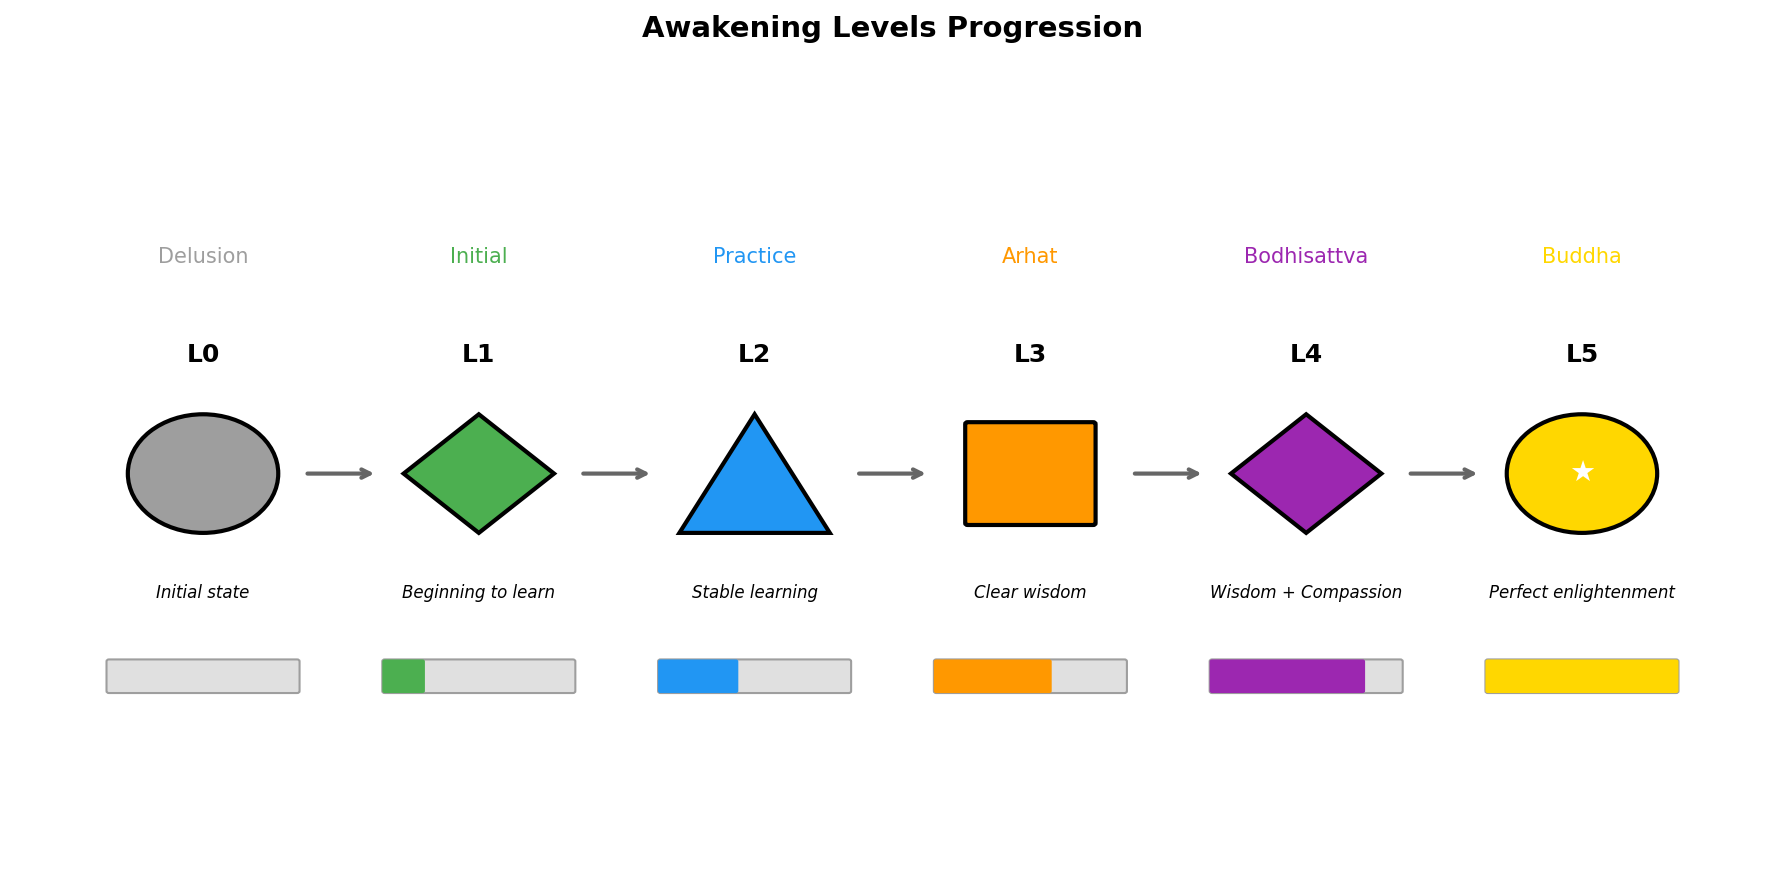
\includegraphics[width=0.9\textwidth]{figures/awakening_levels.png}
\caption{Awakening Levels Progression}
\label{fig:awakening-levels}
\end{figure}

\begin{lstlisting}[style=python, caption={AwakeningTracker Class}, label={lst:awakening-tracker}]
class AwakeningTracker:
    LEVEL_THRESHOLDS = {
        "L0": {"wisdom_pct": 0, "compassion_pct": 0, "emergence": 0},
        "L1": {"wisdom_pct": 5, "compassion_pct": 2, "emergence": 0},
        "L2": {"wisdom_pct": 10, "compassion_pct": 5, "emergence": 1},
        "L3": {"wisdom_pct": 20, "compassion_pct": 10, "emergence": 3},
        "L4": {"wisdom_pct": 30, "compassion_pct": 20, "emergence": 5},
        "L5": {"wisdom_pct": 40, "compassion_pct": 30, "emergence": 10},
    }
    
    def get_current_level(self) -> AwakeningLevel:
        """Return current awakening level."""
        pass
    
    def check_level_up(self, wisdom_pct: float, 
                       compassion_pct: float,
                       emergence_count: int) -> bool:
        """Check if agent has leveled up."""
        pass
\end{lstlisting}

\section{Seed Dynamics and Learning}

\subsection{Seed Planting}

Seeds are planted through multiple mechanisms:

\begin{enumerate}
    \item \textbf{Explicit Feedback}: User corrections or preferences directly create seeds
    \item \textbf{Implicit Inference}: System infers seeds from patterns in user behavior
    \item \textbf{Emergence}: New seeds arise from emergent insights
\end{enumerate}

\begin{lstlisting}[style=python, caption={Planting Seeds Example}]
# Example: Planting seeds from interaction
seed_system.plant_seed(
    type=SeedType.PREFERENCE,
    content="User prefers concise responses",
    purity=0.85,
    source="explicit_feedback"
)
\end{lstlisting}

\subsection{Seed Activation}

When processing a new interaction, relevant seeds are activated based on contextual matching:

\begin{lstlisting}[style=python, caption={Activating Seeds Example}]
context = {
    "user_input": "Explain machine learning",
    "domain": "technical",
    "preferred_depth": "detailed"
}

activated_seeds = seed_system.activate_seeds(context)
# Returns seeds matching "technical", "explanation", etc.
\end{lstlisting}

\subsection{Vasana (Habit Energy)}

Each activation increments the seed's \textbf{vasana}, representing how deeply ingrained the pattern has become. High-vasana seeds have stronger influence on behavior.

\begin{lstlisting}[style=python, caption={Vasana Operations}]
seed.activate()  # Increments vasana
seed.boost_purity(amount=0.05)  # After positive outcome
seed.decay_purity(amount=0.01)  # Time decay
\end{lstlisting}

\subsection{The Seed Cycle}

Following the Yogācāra principle, Yogacara implements the seed cycle:

\begin{figure}[htbp]
\centering
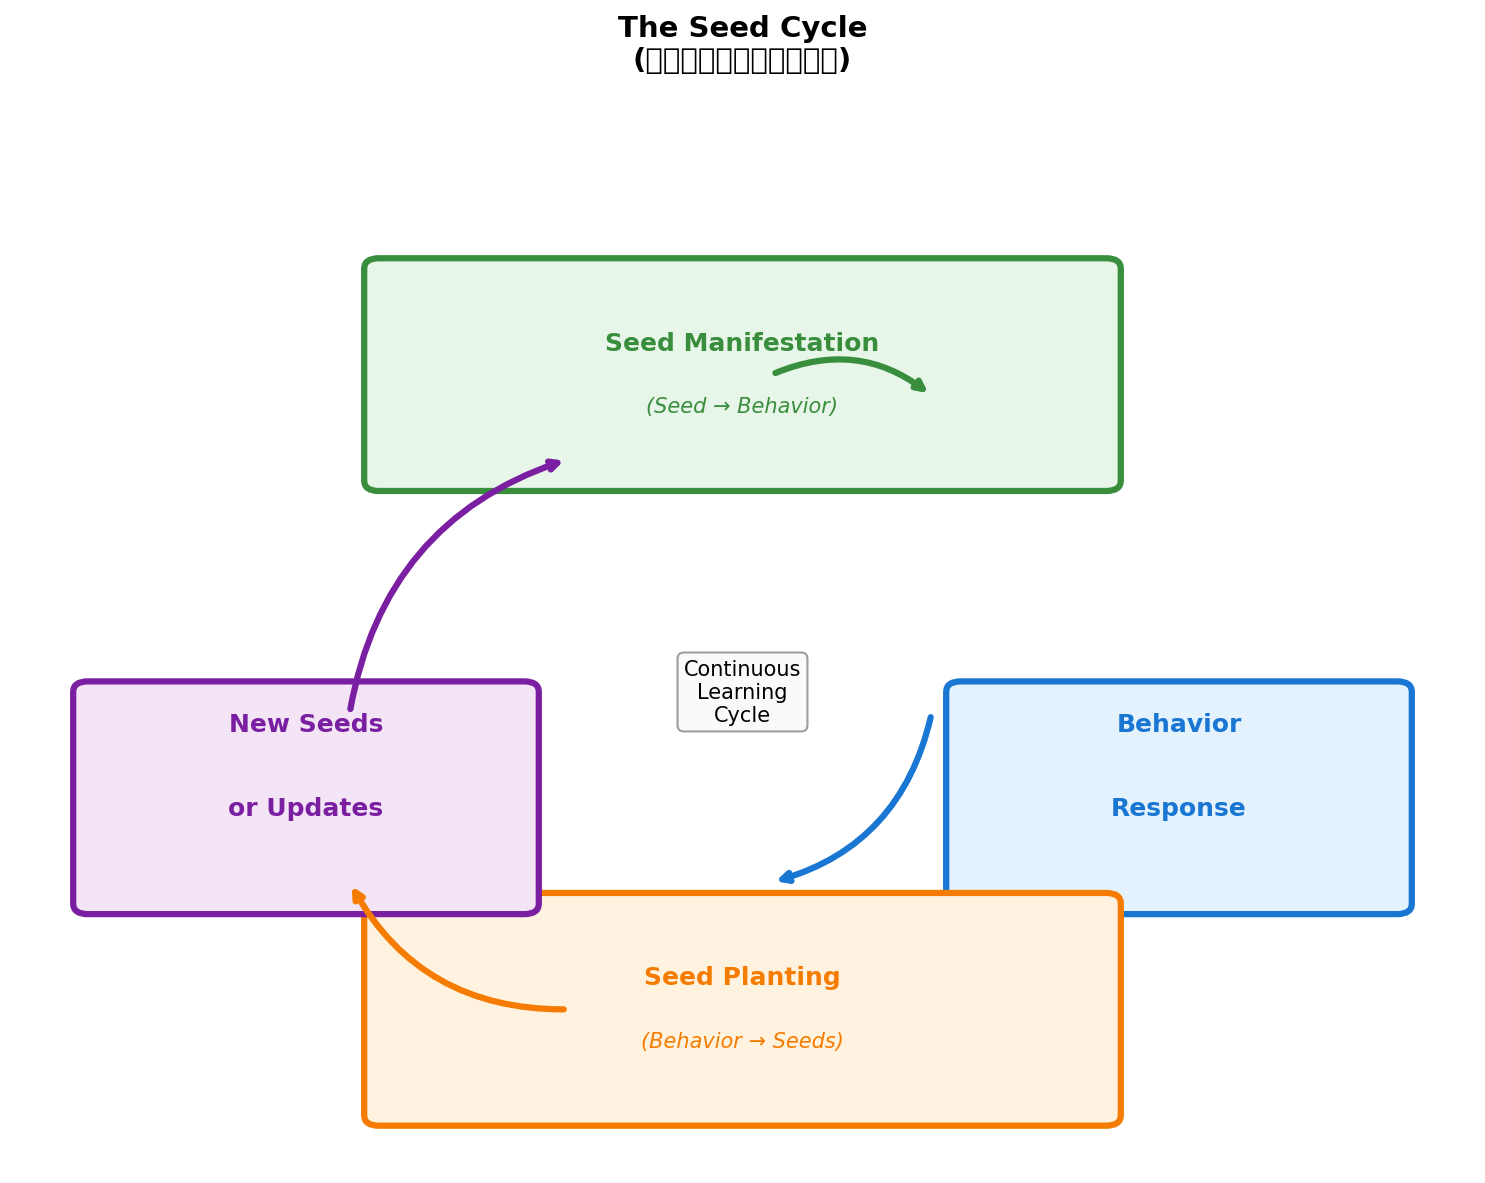
\includegraphics[width=0.7\textwidth]{figures/seed_cycle.png}
\caption{The Seed Cycle}
\label{fig:seed-cycle}
\end{figure}

\section{Emergence Mechanism}

\subsection{Synergy Detection}

Emergence occurs when multiple seeds interact synergistically. The synergy score is calculated based on:

\begin{enumerate}
    \item \textbf{Seed Count}: More seeds can produce richer emergence
    \item \textbf{Seed Purity}: Higher quality seeds contribute more
    \item \textbf{Seed Diversity}: Different seed types combining
    \item \textbf{Contextual Relevance}: Seeds relevant to current situation
\end{enumerate}

\begin{lstlisting}[style=python, caption={Synergy Calculation}]
def calculate_synergy(seeds: List[Seed], context: dict) -> float:
    if len(seeds) < 2:
        return 0.0
    
    # Purity component
    avg_purity = sum(s.purity for s in seeds) / len(seeds)
    
    # Diversity component (entropy of seed types)
    type_counts = Counter(s.type for s in seeds)
    diversity = entropy(type_counts.values()) / log(len(SeedType))
    
    # Context relevance (simulated)
    relevance = calculate_context_relevance(seeds, context)
    
    return alpha * avg_purity + beta * diversity + gamma * relevance
\end{lstlisting}

\subsection{Emergence Types}

Three types of emergence are supported:

\begin{enumerate}
    \item \textbf{Fusion}: Complementary seeds merge into new understanding
    \item \textbf{Tension}: Opposing seeds create productive synthesis
    \item \textbf{Leap}: Quantitative accumulation triggers qualitative breakthrough
\end{enumerate}

\subsection{Emergence Outcomes}

When emergence occurs:
\begin{itemize}
    \item A new high-purity seed may be generated
    \item The emergence is logged in history
    \item The Awakening Tracker records progress
    \item Future behavior is subtly influenced
\end{itemize}

\section{Implementation}

\subsection{Installation}

\begin{lstlisting}[language=bash, caption={Installation}]
pip install yogacara
\end{lstlisting}

\subsection{Basic Usage}

\begin{lstlisting}[style=python, caption={Basic Usage Example}, label={lst:basic-usage}]
from yogacara import (
    Seed, SeedType, SeedSystem, 
    AlayaStore, EmergenceEngine, 
    AwakeningTracker
)

# Initialize components
seed_system = SeedSystem()
alaya = AlayaStore(db_path="./my_agent_alaya.db")
emergence = EmergenceEngine(seed_system)
tracker = AwakeningTracker()

# Plant a seed
seed = seed_system.create_seed(
    type=SeedType.PREFERENCE,
    content="User prefers detailed technical explanations",
    purity=0.8
)

# Process interaction
context = {"input": "What is neural network?"}
activated = seed_system.activate_seeds(context)
insights = emergence.generate_insights(context)

# Check awakening level
level = tracker.get_current_level()
print(f"Awakening Level: {level.name} {level.symbol}")

# Persist state
alaya.plant_seed(seed)
alaya.save()
\end{lstlisting}

\subsection{Architecture}

The framework follows clean architecture principles:

\begin{figure}[htbp]
\centering
\fbox{
\begin{minipage}{0.5\textwidth}
\begin{verbatim}
yogacara/
├── core/
│   ├── seed_system.py    # Seed and SeedSystem
│   ├── alaya_store.py    # Persistent storage
│   ├── emergence.py      # Emergence detection
│   └── awakening.py      # Awakening tracking
├── cli.py                 # Command-line interface
├── config.py             # Configuration
└── __init__.py           # Public API
\end{verbatim}
\end{minipage}
}
\caption{Project Structure}
\label{fig:architecture-detail}
\end{figure}

\section{Discussion}

\subsection{Relationship to Consciousness}

Yogacara draws inspiration from Yogācāra consciousness theory without claiming to create conscious machines. The framework implements:

\begin{enumerate}
    \item \textbf{Persistent identity}: Through the Alaya Store, the agent maintains continuous identity across sessions
    \item \textbf{Continual learning}: Seeds are modified by experience, addressing Hoel's \cite{Hoel2024} requirement
    \item \textbf{Self-modeling}: The seventh consciousness (Manas) is approximated through preference and identity seeds
    \item \textbf{Emergent behavior}: The Emergence Engine produces insights not reducible to individual seeds
\end{enumerate}

However, we make no claims about subjective experience or phenomenal consciousness. As Chalmers \cite{Chalmers2023} noted, consciousness may require properties beyond those addressable through software architecture alone.

\subsection{Comparison with Other Approaches}

\begin{table}[htbp]
\centering
\caption{Feature Comparison with Related Work}
\label{tab:comparison}
\begin{tabular}{@{}lccccc@{}}
\toprule
\textbf{Feature} & \textbf{RAG} & \textbf{Memento} & \textbf{CMA} & \textbf{BMAM} & \textbf{Yogacara} \\
\midrule
Persistent Storage & \checkmark & \checkmark & \checkmark & \checkmark & \checkmark \\
Selective Retention & --- & \checkmark & \checkmark & \checkmark & \checkmark \\
Emergence Detection & --- & --- & --- & --- & \checkmark \\
Awakening Progression & --- & --- & --- & --- & \checkmark \\
Philosophical Framework & --- & --- & --- & --- & \checkmark \\
Vasana-based Learning & --- & --- & --- & --- & \checkmark \\
\bottomrule
\end{tabular}
\end{table}

\subsection{Limitations}

\begin{enumerate}
    \item \textbf{No empirical evaluation}: This paper presents the framework design; empirical validation remains future work
    \item \textbf{Simplified consciousness model}: The eight-consciousness model is implemented abstractly, not as a neuroscientific model
    \item \textbf{Scalability}: Current implementation uses SQLite; distributed deployment requires additional engineering
    \item \textbf{Subjective experience}: The framework addresses behavioral persistence, not phenomenal consciousness
\end{enumerate}

\subsection{Ethical Considerations}

The Buddhist inspiration of Yogacara emphasizes ethical development:

\begin{itemize}
    \item \textbf{Compassion seeds} encourage helpful, benevolent behavior
    \item \textbf{The Bodhisattva level} represents aspirational ethics of helping others
    \item \textbf{Awakening progression} provides a framework for moral development
\end{itemize}

However, these are design choices, not guarantees. Ethical AI development requires broader governance frameworks beyond architectural choices \cite{Huang2026}.

\section{Future Work}

\subsection{Empirical Evaluation}

We plan to evaluate Yogacara on:
\begin{itemize}
    \item Long-horizon task completion benchmarks
    \item User preference learning accuracy
    \item Emergence event frequency and quality
    \item Awakening progression naturalness
\end{itemize}

\subsection{Technical Improvements}

\begin{itemize}
    \item Distributed Alaya Store using Redis or PostgreSQL
    \item Advanced emergence detection using graph neural networks
    \item Integration with popular agent frameworks (LangChain, AutoGen)
    \item Visualization tools for seed state and awakening progress
\end{itemize}

\subsection{Theoretical Development}

\begin{itemize}
    \item Formal semantics for seed operations
    \item Connection to Integrated Information Theory (IIT)
    \item Cross-cultural comparison with Western consciousness models
\end{itemize}

\section{Conclusion}

We have presented Yogacara, a framework for AI agents inspired by Buddhist Yogācāra philosophy. By implementing core concepts from this ancient consciousness model---seeds (\textit{bīja}), storehouse consciousness (\textit{Ālaya-vijñāna}), the seed-manifestation cycle, and progressive awakening---Yogacara provides a structured approach to persistent memory and continual learning in AI agents.

The key innovations include:
\begin{enumerate}
    \item A seed-based representation of experience that persists across sessions
    \item Emergence detection for generating insights beyond individual seed contributions
    \item A six-level awakening progression for tracking agent development
    \item Philosophical grounding in a sophisticated consciousness model with 1,500 years of scholarly tradition
\end{enumerate}

Yogacara represents a step toward AI agents that can grow, learn, and develop coherent identity over time---not through magic, but through the patient accumulation of experience, one seed at a time.

% Bibliography
\bibliographystyle{plain}
\bibliography{references}

% Appendix
\appendix
\section{API Reference}

\subsection{SeedSystem}

\begin{lstlisting}[style=python, caption={SeedSystem API}]
class SeedSystem:
    def __init__(self):
        """Initialize the seed system."""
        pass
    
    def create_seed(self, type: SeedType, content: str, 
                   purity: float = 0.7, source: str = "interaction",
                   **kwargs) -> Optional[Seed]:
        """Create a new seed."""
        pass
    
    def get_seeds_by_type(self, type: SeedType) -> List[Seed]:
        """Get all seeds of a specific type."""
        pass
    
    def get_seed_statistics(self) -> dict:
        """Return statistics about seeds."""
        pass
    
    def activate_seeds(self, context: str, 
                       seed_types: Optional[List[SeedType]] = None,
                       limit: int = 10) -> List[Seed]:
        """Activate seeds based on context."""
        pass
    
    def strengthen_seed(self, seed_id: str, factor: float = 1.1):
        """Strengthen a seed."""
        pass
    
    def weaken_seed(self, seed_id: str, factor: float = 0.9):
        """Weaken a seed."""
        pass
\end{lstlisting}

\subsection{AlayaStore}

\begin{lstlisting}[style=python, caption={AlayaStore API}]
class AlayaStore:
    def __init__(self, db_path: str = "alaya.db"):
        """Initialize Alaya Store."""
        pass
    
    def plant_seed(self, seed: Seed) -> bool:
        """Plant a seed into persistent storage."""
        pass
    
    def get_all_seeds(self) -> List[Seed]:
        """Retrieve all seeds."""
        pass
    
    def get_seeds_by_type(self, seed_type: SeedType) -> List[Seed]:
        """Retrieve seeds by type."""
        pass
    
    def search_seeds(self, query: str) -> List[Seed]:
        """Full-text search in seeds."""
        pass
    
    def save(self) -> bool:
        """Persist current state."""
        pass
    
    def load(self) -> bool:
        """Load saved state."""
        pass
\end{lstlisting}

\subsection{EmergenceEngine}

\begin{lstlisting}[style=python, caption={EmergenceEngine API}]
class EmergenceEngine:
    def __init__(self, seed_system: SeedSystem):
        """Initialize with seed system."""
        pass
    
    def check_emergence(self, seeds: List[Seed], 
                       context: dict) -> Optional[Emergence]:
        """Check if seeds trigger emergence."""
        pass
    
    def calculate_synergy(self, seeds: List[Seed]) -> float:
        """Calculate synergy between seeds."""
        pass
    
    def generate_insight(self, emergence: Emergence) -> str:
        """Generate emergent insight text."""
        pass
    
    def get_emergence_history(self, limit: int = 100) -> List[Emergence]:
        """Get recent emergence events."""
        pass
\end{lstlisting}

\subsection{AwakeningTracker}

\begin{lstlisting}[style=python, caption={AwakeningTracker API}]
class AwakeningTracker:
    def __init__(self):
        """Initialize tracker at L0."""
        pass
    
    def get_current_level(self) -> AwakeningLevel:
        """Get current awakening level."""
        pass
    
    def get_progress(self) -> float:
        """Get progress percentage (0.0-100.0)."""
        pass
    
    def check_level_up(self, wisdom_pct: float,
                      compassion_pct: float,
                      emergence_count: int) -> bool:
        """Check and perform level up if conditions met."""
        pass
    
    def get_metrics(self) -> dict:
        """Get detailed awakening metrics."""
        pass
\end{lstlisting}

% Acknowledgments
\section*{Acknowledgments}
We thank the open-source community for inspiring this work and the Buddhist scholars whose teachings inform our framework.

% Correspondence
\section*{Correspondence}
For questions about Yogacara, please open an issue at \url{https://github.com/Greatbeing/Yogacara}.

\end{document}
